\begin{figure*}[t!]
    \centering
    \begin{subfigure}[b]{0.25\textwidth}
    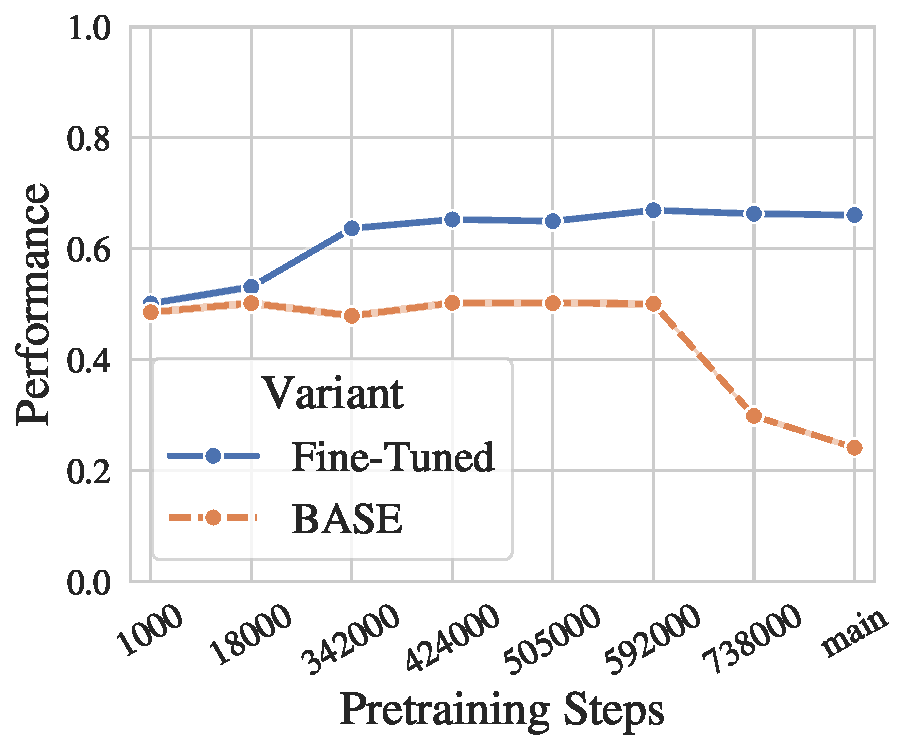
\includegraphics[width=\the\columnwidth]{figures/fig_files/ood/sft_evalrte-trainmnli.pdf}
        \caption{MNLI -> RTE}
    \end{subfigure}%
    ~ 
    \begin{subfigure}[b]{0.25\textwidth}
    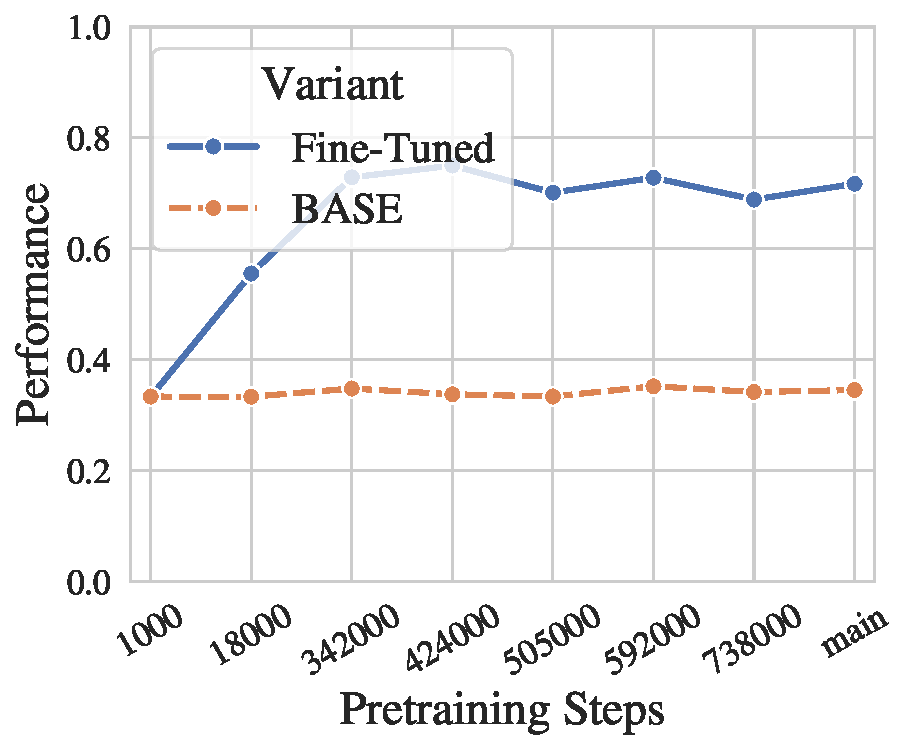
\includegraphics[width=\the\columnwidth]{figures/fig_files/ood/sft_evalgpt3nli-trainmnli.pdf}
        \caption{MNLI -> GPT3NLI}
    \end{subfigure}%
    ~ 
    \begin{subfigure}[b]{0.25\textwidth}
    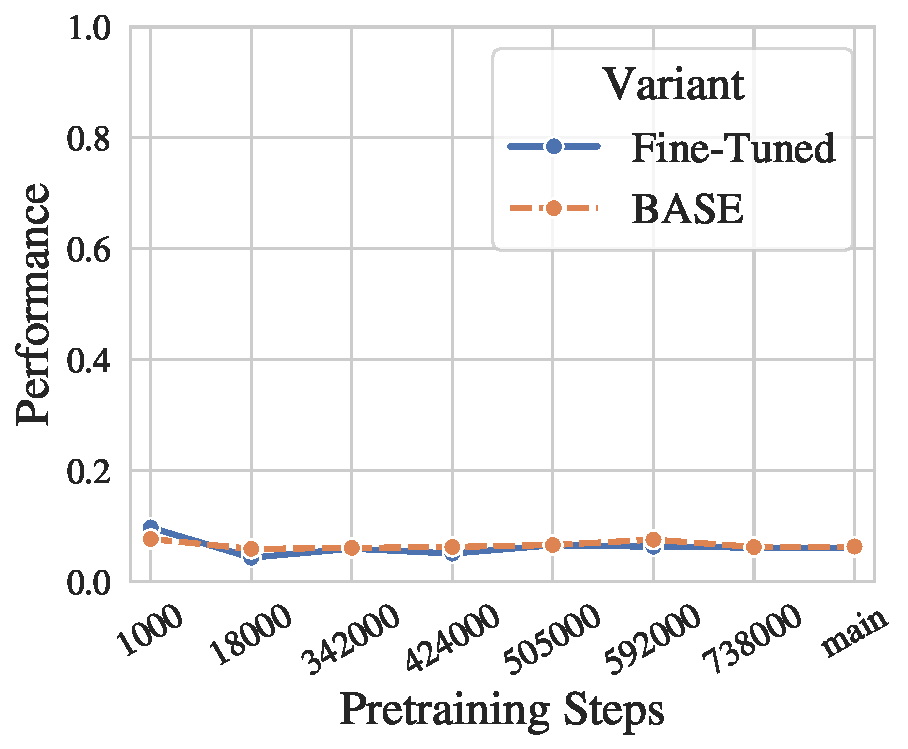
\includegraphics[width=\the\columnwidth]{figures/fig_files/ood/sft_evalcnn-trainxsum.pdf}
        \caption{XSum -> CNN}
    \end{subfigure}%
    \\
    \begin{subfigure}[b]{0.25\textwidth}
    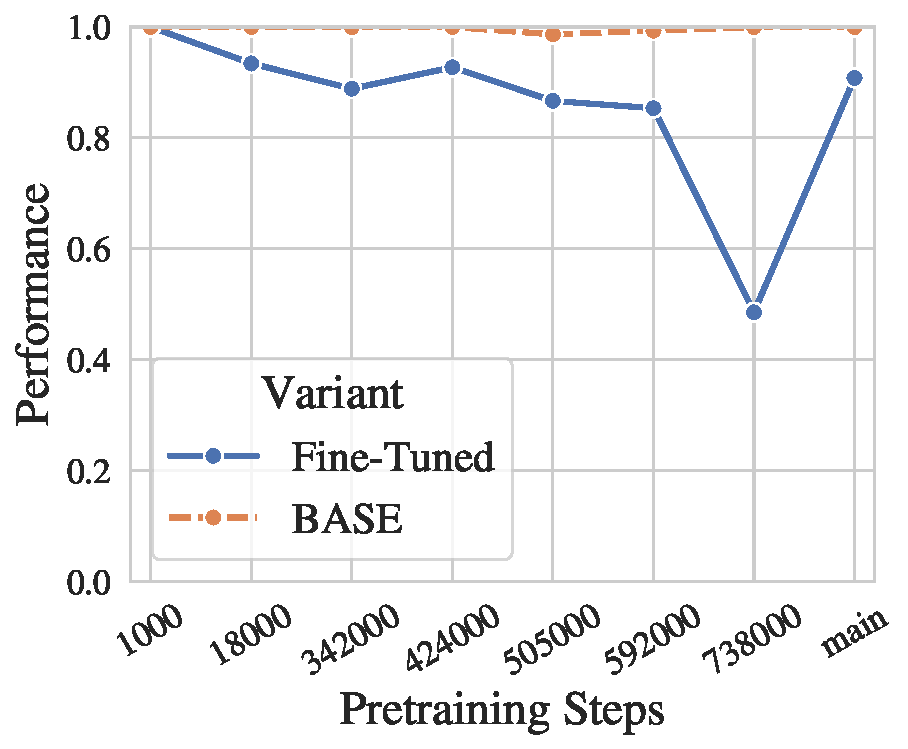
\includegraphics[width=\the\columnwidth]{figures/fig_files/ood/sft_evalqqp-trainpaws.pdf}
        \caption{Paws -> QQP}
    \end{subfigure}%
    ~ 
    \begin{subfigure}[b]{0.25\textwidth}
    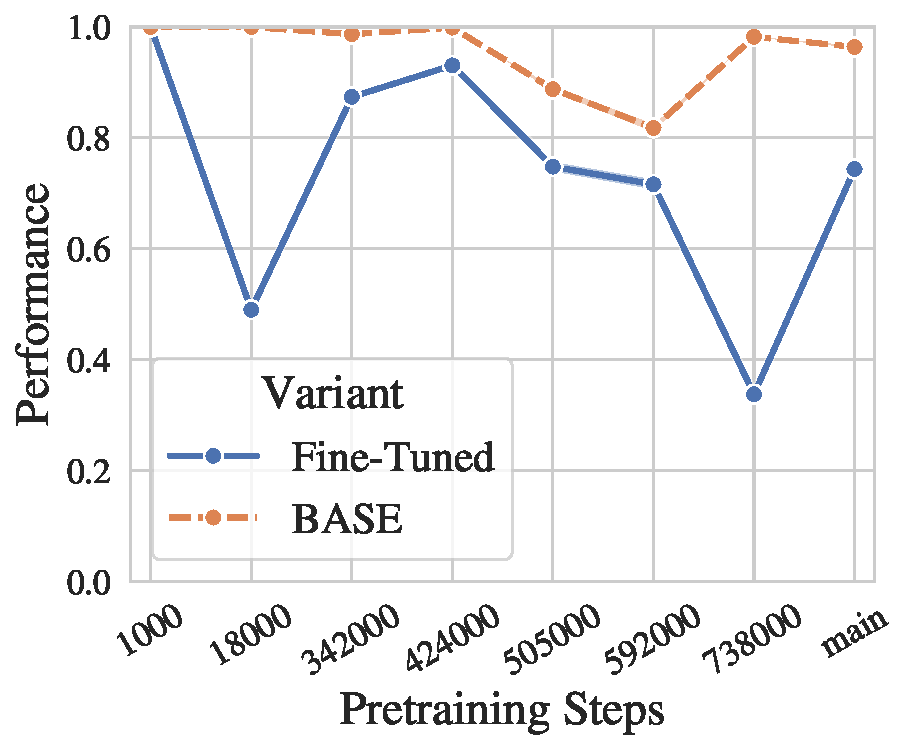
\includegraphics[width=\the\columnwidth]{figures/fig_files/ood/sft_evalstsb-trainpaws.pdf}
        \caption{Paws -> STS-B}
    \end{subfigure}%
    ~ 
    \begin{subfigure}[b]{0.25\textwidth}
    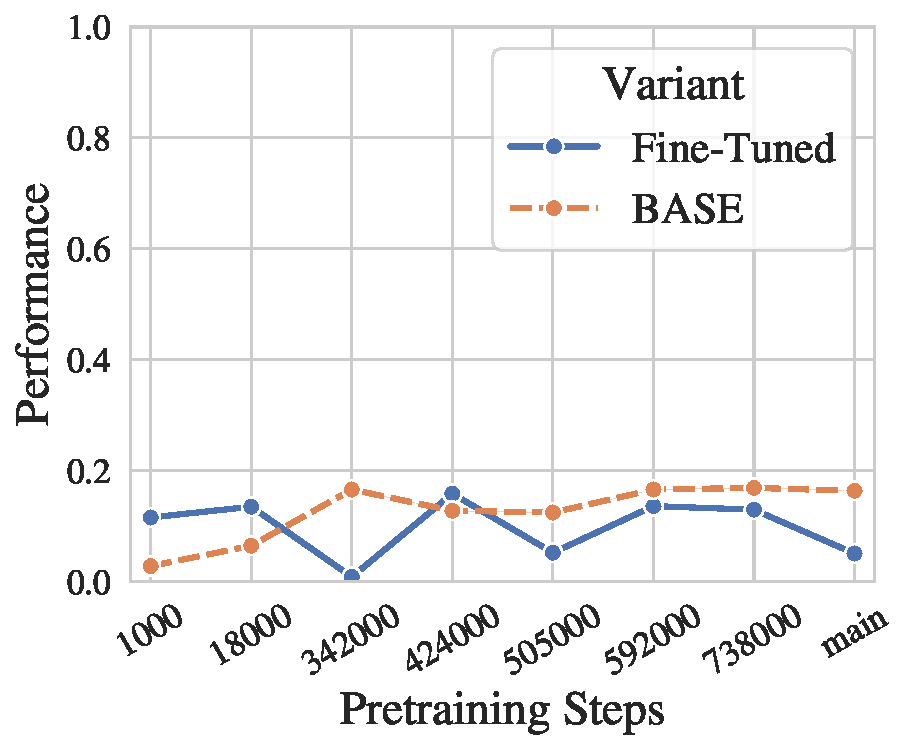
\includegraphics[width=\the\columnwidth]{figures/fig_files/ood/sft_evalsciq-trainsocialiqa.pdf}
        \caption{SocialIQA -> SciQ}
    \end{subfigure}%
    \begin{subfigure}[b]{0.25\textwidth}
    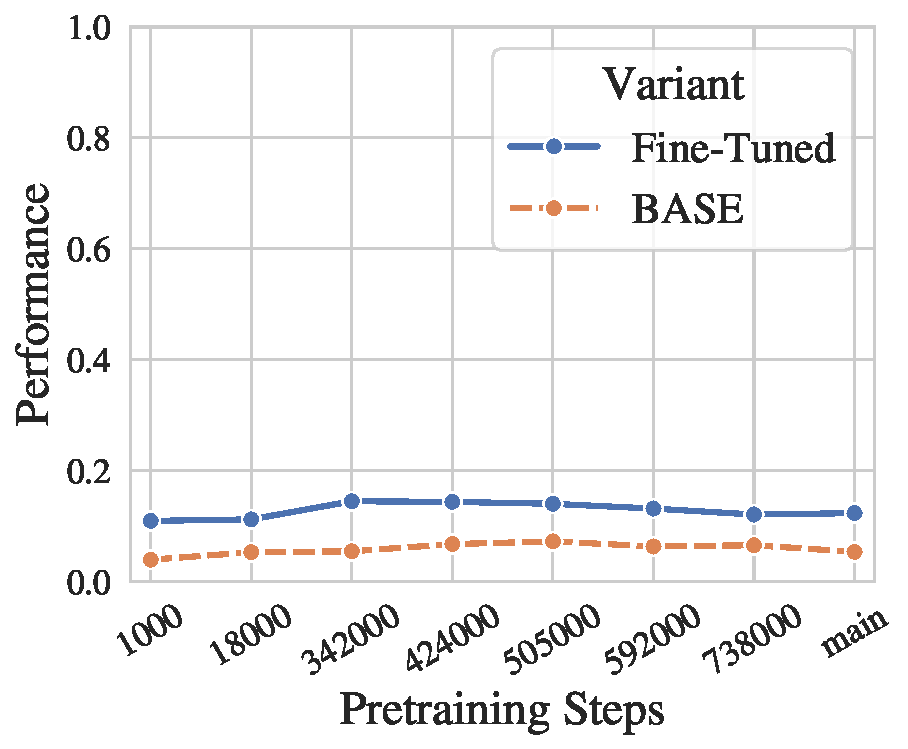
\includegraphics[width=\the\columnwidth]{figures/fig_files/ood/sft_evaltweetqa-trainsocialiqa.pdf}
        \caption{SocialIQA -> TweetQA}
    \end{subfigure}%
    \caption{Out-of-domain performance after supervised fine-tuning on each pre-training step.}
    \label{fig:ood-sft-ckpt-perf}
\end{figure*}